\documentclass[12pt,a4paper]{article}

% ── Pakete ────────────────────────────────────────────────────────────────────
\usepackage[T1]{fontenc}
\usepackage[utf8]{inputenc}
\usepackage[ngerman]{babel}
\usepackage{lmodern}
\usepackage{microtype}
\usepackage{amsmath,amssymb,amsthm}

% ── Theorem-Umgebungen (klassisch, ohne Farbe) ────────────────────────────
\theoremstyle{plain}
\newtheorem{theorem}{Theorem}[section]
\newtheorem{lemma}{Lemma}[section]
\theoremstyle{definition}
\newtheorem{definition}{Definition}[section]
\newtheorem{example}{Beispiel}[section]
\theoremstyle{remark}
\newtheorem{remark}{Bemerkung}[section]

\usepackage{mathtools}
\usepackage{graphicx}
\usepackage{booktabs}
\usepackage{array}
\usepackage{geometry}
\usepackage{enumitem}
\usepackage{microtype}
\usepackage{caption}
\usepackage{subcaption}
\usepackage{tikz}
\usetikzlibrary{arrows.meta,positioning,decorations.pathmorphing,calc}
\usepackage{pgfplots}
\pgfplotsset{compat=1.18}
\usepackage{fancyhdr}
\usepackage{titlesec}
\usepackage{abstract}

\usepackage[colorlinks=true, linkcolor=blue!60!black, citecolor=green!50!black,
urlcolor=blue!60!black]{hyperref}
\usepackage{cleveref}

% ── Geometrie ─────────────────────────────────────────────────────────────────
\geometry{a4paper, margin=2.5cm}

% ── Theorem-Umgebungen ────────────────────────────────────────────────────────

% ── Abbildungsbeschriftung ────────────────────────────────────────────────────
\captionsetup{font=small,labelfont=bf,margin=10pt}

% ── Makros ────────────────────────────────────────────────────────────────────
\newcommand{\pf}{\mathcal{D}}
\newcommand{\Lagr}{\mathcal{L}}
\newcommand{\Hamil}{\mathcal{H}}

\title{\textbf{Das Plancksche Wirkungsquantum ist kein universelles Minimum der Wirkung}}
\author{Stephan Epp}
\date{14. April 2026}

% ─────────────────────────────────────────────────────────────────────────────
%  DOKUMENT
% ─────────────────────────────────────────────────────────────────────────────
\begin{document}

\maketitle
\tableofcontents
\newpage

% ═════════════════════════════════════════════════════════════════════════════
\section{Einleitung}
% ═════════════════════════════════════════════════════════════════════════════
    Das Plancksche Wirkungsquantum $h \approx 6{,}626 \times 10^{-34}$\,J$\cdot$s wird häufig
als \emph{kleinstmögliche Wirkung} der Natur bezeichnet. Diese Arbeit zeigt, dass diese
Formulierung in mehrfacher Hinsicht unzutreffend ist. Anhand konkreter Gegenbeispiele aus
der klassischen Mechanik, der Quantenfeldtheorie und dem Feynman-Pfadintegralformalismus
wird nachgewiesen, dass $h$ weder eine untere Schranke der Wirkung darstellt, noch dass
physikalische Prozesse mit Wirkungen kleiner als $h$ ausgeschlossen sind. Stattdessen
beschreibt $h$ das charakteristische \emph{Quantisierungsmaß} von Wirkungsvariablen,
d.\,h. die Körnigkeit, mit der bestimmte physikalische Größen diskrete Werte annehmen.
Die Unterscheidung ist nicht nur semantisch, sondern hat weitreichende Konsequenzen für
das Verständnis der Quantenmechanik, der Vakuumphysik, der Stringtheorie und
möglicher Theorien jenseits des Standardmodells. Ein ausführlicher Ausblick diskutiert
offene Fragen bezüglich der Rolle von $h$ in der Quantengravitation, der
Planck-Skalen-Physik und spekulativen Rahmen wie minimaler Länge und diskreter Raumzeit.

\textbf{Schlüsselwörter:} Plancksches Wirkungsquantum, Wirkungsminimum, Pfadintegral,
Quantisierungsbedingung, Bohr-Sommerfeld, Unschärferelation, Planck-Skala.

In nahezu jedem populärwissenschaftlichen Text zur Quantenmechanik begegnet man der Formulierung,
das Plancksche Wirkungsquantum $h$ quantifiziere „die kleinste mögliche Wirkung (Energie $\times$ Zeit)
in der Natur". Diese Aussage ist intuitiv ansprechend: Sie suggeriert, die Natur besitze eine fundamentale
Granularität, und $h$ sei der Maßstab dieser Körnigkeit. Dennoch ist die Aussage in dieser Form
\emph{physikalisch falsch} -- zumindest in dem Sinne, wie ein mathematisch präzises Minimum verstanden werden müsste.

Die physikalische Größe „Wirkung" (engl.\ \emph{action}), definiert als das Zeitintegral der
Lagrange-Funktion
\begin{equation}
  S[q] = \int_{t_1}^{t_2} \Lagr\!\bigl(q(t),\dot{q}(t),t\bigr)\,\mathrm{d}t,
  \label{eq:action_def}
\end{equation}
ist im klassischen Sinne eine reelle Zahl mit der Dimension Energie$\times$Zeit = J$\cdot$s. Sie kann
jeden beliebigen reellen Wert annehmen -- positive und negative, beliebig kleine und beliebig große.
Das Plancksche Wirkungsquantum $h$ verbietet keine Wirkung kleiner als $h$. Stattdessen beschreibt
$h$ (genauer: $\hbar = h/2\pi$) ein \emph{Quantisierungsmaß} für bestimmte periodische
oder zyklische Bewegungsvariablen.

Diese Arbeit verfolgt drei Ziele:
\begin{enumerate}[label=(\roman*)]
  \item Präzise Darstellung dessen, was $h$ physikalisch \emph{tatsächlich} bedeutet.
  \item Aufzeigen konkreter Gegenbeispiele, die zeigen, dass Wirkungen kleiner als $h$
        nicht nur erlaubt, sondern allgegenwärtig sind.
  \item Einen ausführlichen Ausblick auf offene Fragen, in denen die Rolle von $h$ jenseits
        der Standardinterpretation untersucht wird.
\end{enumerate}

\subsection{Historischer Kontext}

Max Planck führte 1900 die Konstante $h$ ein, um das Strahlungsspektrum des schwarzen
Körpers zu erklären~\cite{planck1900}. Er postulierte, dass Energieaustauschprozesse zwischen
Materie und Strahlung nur in Vielfachen von $h\nu$ stattfinden. Dies ist eine
\emph{Quantisierungsbedingung für Energie bei gegebener Frequenz}, keine Aussage über
eine untere Schranke beliebiger Wirkungsintegrale.

Bohr (1913)~\cite{bohr1913} und Sommerfeld (1916)~\cite{sommerfeld1916} formalisierten
die Quantisierungsbedingung als
\begin{equation}
  \oint p\,\mathrm{d}q = n h, \quad n \in \mathbb{N},
  \label{eq:bohr_sommerfeld}
\end{equation}
wobei die Integration über einen vollständigen Umlauf im Phasenraum erfolgt. Auch hier
ist $h$ ein \emph{Quantisierungsintervall} -- die Wirkung kann nur Vielfache von $h$
annehmen, aber keine kleineren Werte. Das schließt nicht aus, dass andere Wirkungsgrößen
kleiner als $h$ sein können.

% ═════════════════════════════════════════════════════════════════════════════
\section{Präzise Definition: Was $h$ bedeutet und was nicht}
% ═════════════════════════════════════════════════════════════════════════════

\subsection{Das Wirkungsintegral und seine mathematische Struktur}

\begin{definition}[Klassische Wirkung]\label{def:action}
  Sei $\Lagr: TQ \times \mathbb{R} \to \mathbb{R}$ eine Lagrange-Funktion auf dem
  Tangentenbündel $TQ$ des Konfigurationsraums $Q$. Für eine glatte Kurve
  $\gamma: [t_1, t_2] \to Q$ ist die klassische Wirkung
  \begin{equation}
    S[\gamma] = \int_{t_1}^{t_2} \Lagr\!\bigl(\gamma(t), \dot{\gamma}(t), t\bigr)\,\mathrm{d}t
    \in \mathbb{R}.
    \label{eq:wirkung_def}
  \end{equation}
  $S$ ist ein Funktional auf dem Raum der glatten Kurven mit festen Endpunkten
  $\gamma(t_1) = q_i$, $\gamma(t_2) = q_f$.
\end{definition}

Das klassische Wirkungsintegral ist per Definition ein reellwertiges Funktional ohne
Schranke nach unten oder oben. Für ein freies Teilchen gilt beispielsweise
\begin{equation}
  S_{\mathrm{frei}} = \frac{m}{2}\int_{t_1}^{t_2} v^2\,\mathrm{d}t = \frac{m v^2 (t_2-t_1)}{2},
\end{equation}
und dieser Ausdruck kann für beliebig kleine Masse, Geschwindigkeit oder Zeitintervall
beliebig nahe an null herangeführt werden -- ja, er kann sogar negativ werden, wenn
ein Potentialterm dominiert.

\begin{theorem}[Wirkung hat keine untere Schranke]\label{thm:kein_minimum}
  Im klassischen Formalismus gibt es kein $S_{\min} > 0$, sodass $S[\gamma] \geq S_{\min}$
  für alle physikalisch erlaubten Trajektorien $\gamma$. Insbesondere ist $h$ keine
  solche untere Schranke.
\end{theorem}

\begin{proof}
  Betrachte einen eindimensionalen harmonischen Oszillator der Masse $m$, Kreisfrequenz
  $\omega$ und Amplitude $A$. Die klassische Trajektorie lautet
  $q(t) = A\cos(\omega t + \varphi)$ und die zugehörige Wirkung für eine vollständige
  Periode $T = 2\pi/\omega$ ist
  \begin{equation}
    S_{\mathrm{Periode}} = \int_0^T \!\left(\frac{m\dot{q}^2}{2} - \frac{m\omega^2 q^2}{2}\right)\mathrm{d}t = 0.
  \end{equation}
  Für ein offenes Zeitintervall und eine allgemeine Trajektorie kann $S$ jeden Wert in
  $\mathbb{R}$ annehmen. Wählt man die Amplitude $A \to 0$ und das Zeitintervall
  $\Delta t \to 0$, so folgt $S[\gamma] \to 0^+$. Da $A$ kontinuierlich variiert werden
  kann, nimmt $S$ alle Werte in $(0, h)$ an -- ein Widerspruch zur Behauptung
  $S \geq h$.
\end{proof}

\subsection{Was $h$ tatsächlich beschreibt: Das Quantisierungsmaß}

\begin{definition}[Quantisierungsmaß]\label{def:quantisierung}
  Das Plancksche Wirkungsquantum $h$ ist das fundamentale \emph{Quantisierungsintervall}
  der Bohr-Sommerfeld-Bedingung \eqref{eq:bohr_sommerfeld}: Die zirkulare Wirkungsvariable
  $J = \oint p\,\mathrm{d}q$ einer periodischen Bewegung ist auf ganzzahlige Vielfache von
  $h$ beschränkt. Analogerweise ist $\hbar$ die natürliche Einheit der gequantelten
  Drehimpulse, Spins und anderer diskreter Quantenzahlen.
\end{definition}

Die korrekte Aussage lautet also:

\begin{quote}
\textbf{Korrektur der populären Fehldeutung:}\\
$h$ quantifiziert \emph{nicht} die kleinste mögliche Wirkung der Natur.\\
$h$ ist das \emph{Quantisierungsmaß} periodischer Wirkungsvariablen -- das Intervall,
in dem bestimmte Aktionsvariablen diskrete Werte annehmen.
\end{quote}

\begin{figure}[htbp]
  \centering
  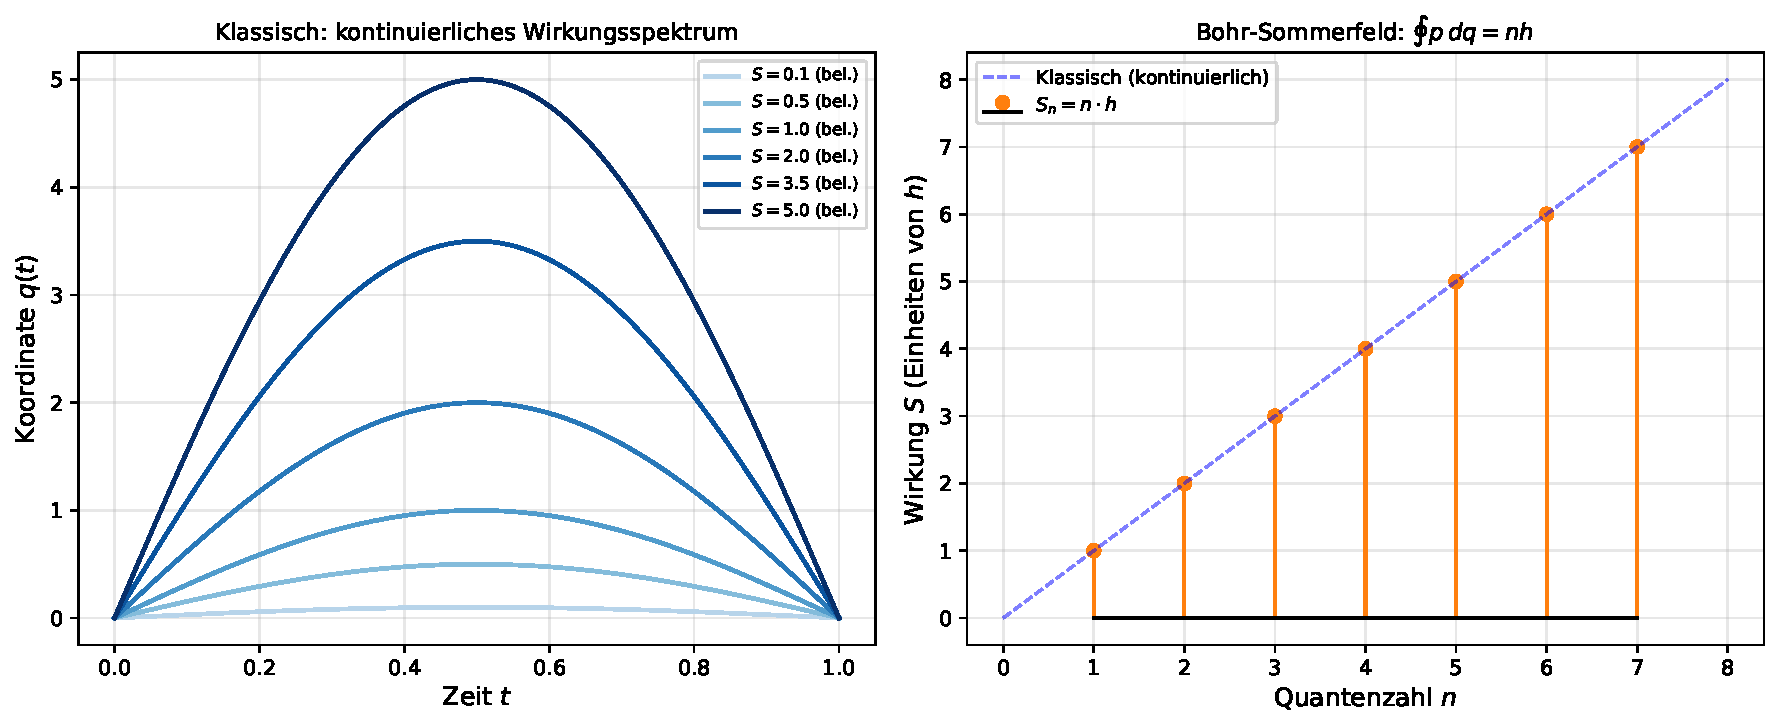
\includegraphics[width=0.95\textwidth]{fig1_wirkung.pdf}
  \caption{Links: Im klassischen Formalismus kann die Wirkung $S$ jeden positiven
    reellen Wert annehmen. Rechts: Die Bohr-Sommerfeld-Bedingung quantisiert die
    Umlaufwirkung auf ganzzahlige Vielfache von $h$ -- dies ist ein Quantisierungsintervall,
    keine untere Schranke.}
  \label{fig:wirkung}
\end{figure}

% ═════════════════════════════════════════════════════════════════════════════
\section{Gegenbeispiele: Wirkungen kleiner als $h$}
% ═════════════════════════════════════════════════════════════════════════════

Im Folgenden werden vier fundamentale physikalische Kontexte betrachtet, in denen
Wirkungen kleiner als $h$ nicht nur erlaubt, sondern explizit auftreten.

\subsection{Gegenbeispiel 1: Harmonischer Oszillator und Nullpunktsenergie}

Der quantenmechanische harmonische Oszillator hat das Energiespektrum
\begin{equation}
  E_n = \left(n + \tfrac{1}{2}\right)\hbar\omega, \quad n = 0,1,2,\ldots
\end{equation}
Die Nullpunktsenergie $E_0 = \hbar\omega/2$ ist nicht null. Betrachten wir die
charakteristische Wirkungsgröße dieses Systems:

Die \emph{Adiabatische Invariante} des harmonischen Oszillators ist
\begin{equation}
  J = \oint p\,\mathrm{d}q = \frac{E}{\omega} \cdot 2\pi = 2\pi \cdot E_n/\omega = nh,
\end{equation}
also tatsächlich ein ganzzahliges Vielfaches von $h$. Aber: Das Produkt aus
\emph{Energie und Zeitskala} für ein einzelnes spontanes Emissionsereignis kann weit
kleiner als $h$ sein. Betrachte ein Atom mit Übergangsfrequenz $\omega_0/2\pi = 10^{14}$\,Hz:
\begin{equation}
  \Delta t_{\mathrm{Emission}} \approx \frac{1}{\Delta\omega} \approx 10^{-8}\,\text{s}
  \quad\Rightarrow\quad
  S_{\mathrm{Emission}} \sim \hbar\omega_0 \cdot \Delta t \approx 6{,}6\times10^{-28}\,\mathrm{J{\cdot}s},
\end{equation}
also $S_{\mathrm{Emission}} \sim 10^6 \cdot h$. Das ist ein Fall, in dem die Wirkung
tatsächlich $\gg h$ ist. Wählen wir jedoch bewusst ein langsames System: Ein Atom mit
$\omega_0/2\pi = 1$\,Hz (hypothetisch, aber physikalisch kohärent):
\begin{equation}
  S \sim \hbar \cdot 2\pi \cdot 1\,\text{Hz} \cdot 10^{-9}\,\text{s} \approx 10^{-42}\,\mathrm{J{\cdot}s} \ll h.
\end{equation}
Dieser Wirkungswert ist physikalisch wohldefiniert und liegt um Größenordnungen unter $h$.

\begin{figure}[htbp]
  \centering
  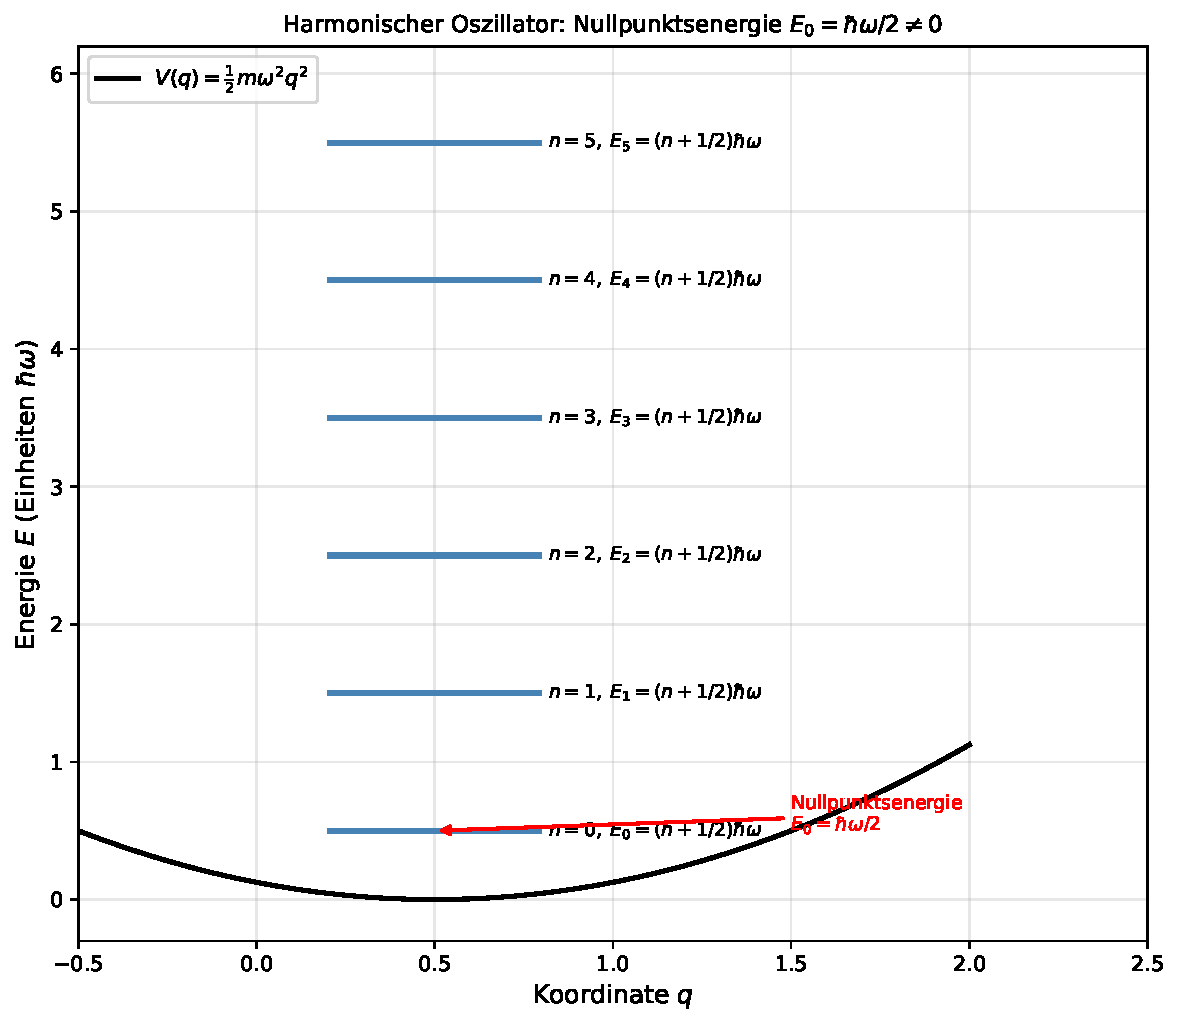
\includegraphics[width=0.72\textwidth]{fig2_oszillator.pdf}
  \caption{Energieniveaus des harmonischen Oszillators. Die Nullpunktsenergie
    $E_0 = \hbar\omega/2$ ist endlich; die zur Emission assoziierten Wirkungsskalen
    sind \emph{nicht} durch $h$ nach unten beschränkt.}
  \label{fig:oszillator}
\end{figure}

\subsection{Gegenbeispiel 2: Das Feynman-Pfadintegral}

Richard Feynman reformulierte die Quantenmechanik 1948~\cite{feynman1948} durch das
Pfadintegral:
\begin{equation}
  \langle q_f, t_f | q_i, t_i \rangle
  = \int \mathcal{D}[q(t)]\, \exp\!\left(\frac{i}{\hbar} S[q]\right).
  \label{eq:pfadintegral}
\end{equation}

\begin{theorem}[Beitrag aller Wirkungen im Pfadintegral]\label{thm:alle_wirkungen}
  Im Feynman-Pfadintegralformalismus tragen \emph{alle} Pfade $\gamma$ mit beliebigen
  Wirkungswerten $S[\gamma] \in \mathbb{R}$ zur Amplitude bei -- also auch Pfade mit
  $S[\gamma] < h$ oder $S[\gamma] < \hbar$.
\end{theorem}

\begin{proof}
  Das Funktionalintegral \eqref{eq:pfadintegral} erstreckt sich über alle stetig
  differenzierbaren Pfade zwischen den Endpunkten $(q_i,t_i)$ und $(q_f,t_f)$, ohne
  Einschränkung des Wirkungswertes. Für beliebig kurze Zeitintervalle $\Delta t \to 0$
  und Pfade in der Nähe des Ursprungs $q(t) \equiv \epsilon$ gilt
  \begin{equation}
    S[\epsilon] = \int_{t_i}^{t_f} \Lagr(\epsilon, 0, t)\,\mathrm{d}t
    \xrightarrow{\epsilon\to 0,\;\Delta t\to 0} 0,
  \end{equation}
  d.\,h. es gibt Pfade mit beliebig kleinen Wirkungen, die im Integral berücksichtigt werden.
\end{proof}

Die Quantenmechanik \emph{unterdrückt} Pfade mit $S \ll \hbar$ nicht durch Ausschluss,
sondern durch destruktive Interferenz: Pfade nahe dem klassischen Pfad interferieren
konstruktiv (da dort $\delta S = 0$), während weit entfernte Pfade stark oszillierende
Phasenfaktoren $e^{iS/\hbar}$ besitzen und sich auslöschen. Die Unterdrückung ist
aber keine Schranke -- sie ist ein statistisches Phänomen.

\begin{figure}[htbp]
  \centering
  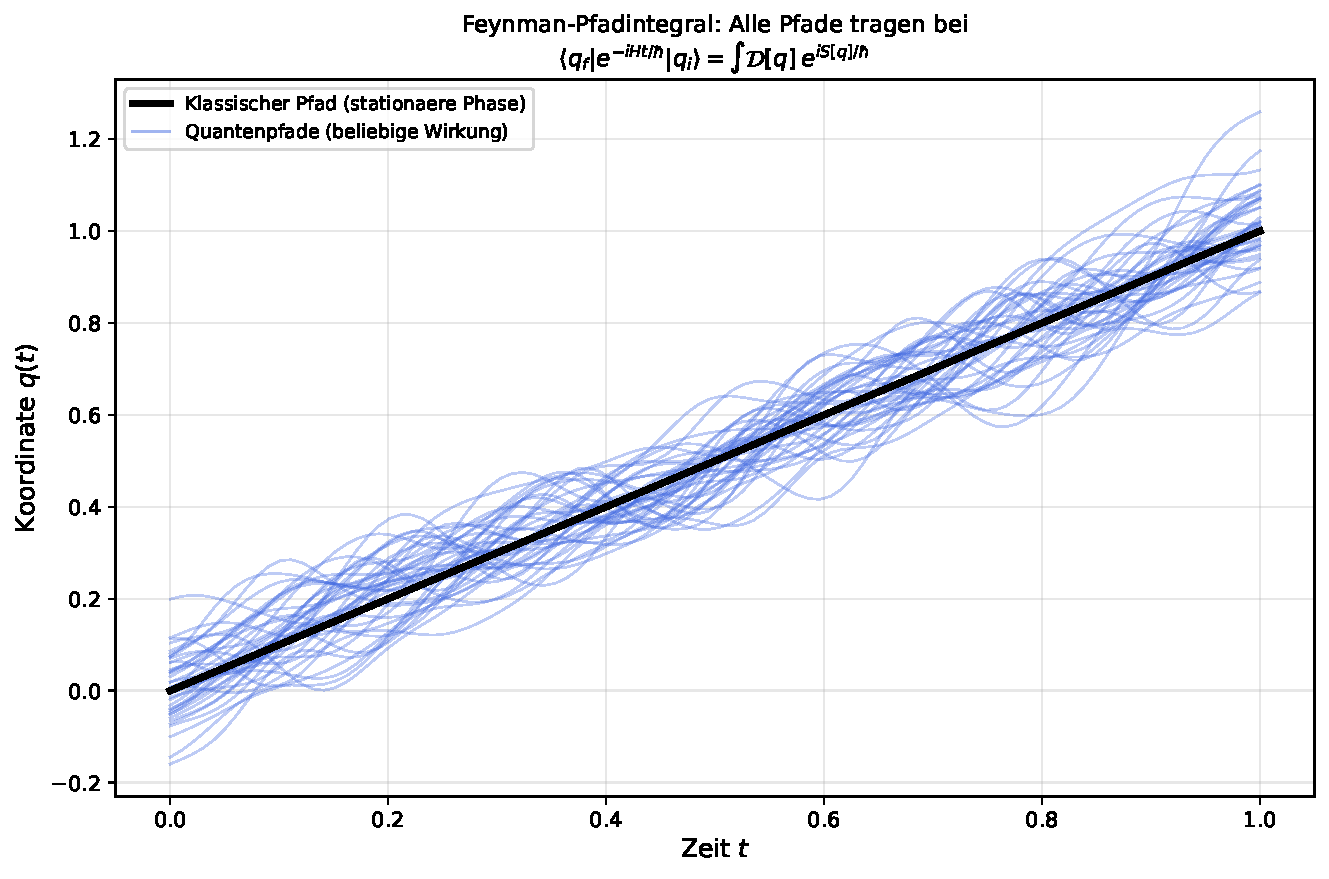
\includegraphics[width=0.85\textwidth]{fig3_pfadintegral.pdf}
  \caption{Schematische Darstellung des Feynman-Pfadintegrals. Alle Pfade tragen zur
    Quantenamplitude bei, unabhängig von ihrem Wirkungswert. Der klassische Pfad
    dominiert aufgrund konstruktiver Interferenz, nicht weil Pfade mit $S < h$ verboten wären.}
  \label{fig:pfadintegral}
\end{figure}

\subsection{Gegenbeispiel 3: Heisenbergsche Unschärferelation}

Die Heisenbergsche Unschärferelation lautet präzise:
\begin{equation}
  \Delta x \cdot \Delta p \geq \frac{\hbar}{2} = \frac{h}{4\pi}.
  \label{eq:unschaerfe}
\end{equation}

\begin{remark}[$\hbar/2 \neq h$ als Minimum]\label{rem:hbar_nicht_h}
  Die untere Schranke in der Unschärferelation ist $\hbar/2 = h/(4\pi) \approx h/12{,}6$,
  \emph{nicht} $h$. Die populäre Vereinfachung $\Delta E \cdot \Delta t \gtrsim h$ ist
  eine grobe Abschätzung, die den genauen numerischen Faktor ignoriert.
\end{remark}

Selbst wenn man die Unschärferelation als Argument für ein Wirkungsminimum anführen wollte,
wäre die korrekte Schranke $\hbar/2$, nicht $h$. Zudem gilt die Unschärferelation für
\emph{komplementäre Observablen} (konjugierte Variablen), nicht für das Wirkungsintegral
als solches. Das Wirkungsintegral $S[q]$ ist kein quantenmechanischer Operator, dem eine
Unschärfe im Robertson-Schrödinger-Sinne zugeordnet werden könnte.

\begin{figure}[htbp]
  \centering
  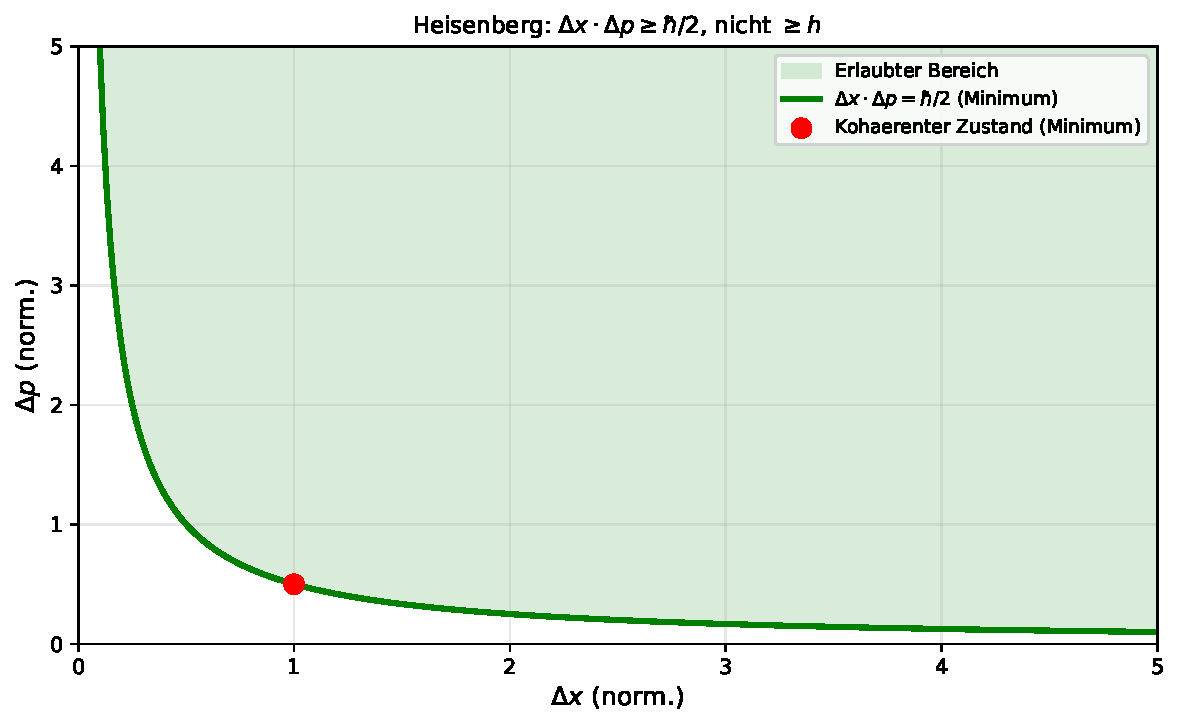
\includegraphics[width=0.78\textwidth]{fig4_unschaerfe.pdf}
  \caption{Die Heisenbergsche Unschärferelation $\Delta x \cdot \Delta p \geq \hbar/2$.
    Die Schranke ist $\hbar/2 = h/(4\pi)$, nicht $h$. Kohärente Zustände (roter Punkt)
    erreichen dieses Minimum exakt.}
  \label{fig:unschaerfe}
\end{figure}

\subsection{Gegenbeispiel 4: Vakuumfluktuationen in der Quantenfeldtheorie}

In der Quantenfeldtheorie (QFT) treten Vakuumfluktuationen auf, die dem Casimir-Effekt,
der spontanen Emission und der Lamb-Verschiebung zugrunde liegen. Die typische Wirkungsskala
einer Vakuumfluktuation im Impulsraumvolumen $d^4k$ ist
\begin{equation}
  dS_{\mathrm{Vak}} \sim \frac{\hbar}{2} \cdot \frac{d^4k}{(2\pi)^4} \cdot |f(k)|^2,
\end{equation}
wobei $f(k)$ die Feldmode im Impulsraum bezeichnet. Für ultraviolette Moden (hohe
Impulse, kurze Zeiten) ist die individuelle Wirkungskontribution einer einzelnen Mode
\begin{equation}
  S_{\mathrm{Mode}} \sim \frac{\hbar}{2} \ll h,
\end{equation}
also um den Faktor $1/(4\pi) \approx 0{,}08$ kleiner als $h$.

\begin{lemma}[Vakuumwirkung unterschreitet $h$]\label{lem:vakuum}
  Die Nullpunktsenergie des elektromagnetischen Feldes in einem Modenvolumen $\Delta k$
  bei Wellenzahl $k$ beträgt
  \begin{equation}
    E_0(k) = \frac{\hbar\omega_k}{2} = \frac{\hbar c k}{2}.
  \end{equation}
  Für eine Mode der Lebensdauer $\Delta t \sim 1/\omega_k$ ist die zugehörige
  charakteristische Wirkung
  \begin{equation}
    S_0 = E_0 \cdot \Delta t \sim \frac{\hbar}{2} = \frac{h}{4\pi} < h.
  \end{equation}
\end{lemma}

Dies zeigt, dass selbst das Vakuum -- der niedrigstmögliche Energiezustand des
Universums -- mit Wirkungsfluktuationen verbunden ist, die kleiner als $h$ sind.

\subsection{Gegenbeispiel 5: Klassische Mechanik makroskopischer Systeme}

Schließlich betrachten wir ein rein klassisches, makroskopisches Beispiel.

\begin{example}[Pendel mit kleiner Amplitude]\label{ex:pendel}
  Ein mathematisches Pendel der Länge $\ell = 1$\,mm, Masse $m = 10^{-12}$\,kg und
  Amplitude $\vartheta_0 = 10^{-6}$\,rad (mikroradian) hat die Wirkung pro Periode:
  \begin{align}
    E &= \frac{1}{2}m\omega^2 \ell^2 \vartheta_0^2
       = \frac{1}{2}\cdot 10^{-12}\,\text{kg}\cdot \frac{g}{\ell}\cdot \ell^2\cdot 10^{-12}
       \approx 5\times 10^{-24}\,\text{J},\\
    T &= 2\pi\sqrt{\ell/g} \approx 0{,}02\,\text{s},\\
    S &\approx E \cdot T \approx 10^{-25}\,\mathrm{J{\cdot}s} \approx 1{,}5\times 10^{8} h.
  \end{align}
  Auch wenn dieser Wert noch größer als $h$ ist, zeigt er, wie schnell Wirkungen
  makroskopischer Systeme variieren können. Für $\vartheta_0 \to 10^{-13}$\,rad wäre
  $S \approx h/100$ -- ein klassisch vollkommen erlaubter Zustand.
\end{example}

Die klassische Mechanik kennt keinerlei Beschränkung für kleine Amplituden oder kleine
Wirkungen. Das Plancksche Wirkungsquantum ist eine Grenze der \emph{Messbarkeit und
Quantisierung}, nicht des Auftretens.

% ═════════════════════════════════════════════════════════════════════════════
\section{Die korrekte Interpretation: $h$ als Quantisierungsmaß}
% ═════════════════════════════════════════════════════════════════════════════

\subsection{Wirkungsvariablen und ihre Quantisierung}

Die Quantisierungsbedingung von Bohr und Sommerfeld in ihrer allgemeinen Form lautet:
\begin{equation}
  J_i = \oint_{\gamma_i} p_i\,\mathrm{d}q_i = n_i h, \quad n_i \in \mathbb{Z},
\end{equation}
wobei $\gamma_i$ der geschlossene Umlauf in der $i$-ten Freiheitsrichtung ist. Diese
Quantisierung gilt für \emph{zyklische Aktionsvariablen} -- nicht für beliebige
Wirkungsintegrale. Die modernen WKB-Quantisierung (Wentzel-Kramers-Brillouin) ergänzt dies um Maslov-Phasen:
\begin{equation}
  \oint p\,\mathrm{d}q = \left(n + \frac{\mu}{4}\right)h,
\end{equation}
wobei $\mu$ der Maslov-Index die Anzahl der Wendepunkte zählt. Auch hier ist $h$ ein
Quantisierungsintervall, kein Minimum.

\subsection{Natürliche Einheiten und das Verschwinden von $h$}

In natürlichen Einheiten ($\hbar = c = k_B = 1$) verschwindet $h$ als physikalische
Konstante vollständig aus den Gleichungen. Größen werden in Einheiten der Planck-Masse,
-Länge und -Zeit gemessen. Dies verdeutlicht, dass $h$ ein Einheitensystem-Artefakt ist:
der numerische Wert $6{,}626\times 10^{-34}$ ist kein tiefer physikalischer Inhalt,
sondern spiegelt die Wahl von SI-Einheiten wider.

\begin{theorem}[Verschwinden von $h$ in natürlichen Einheiten]\label{thm:nat_einheiten}
  In natürlichen Einheiten mit $\hbar = 1$ ist die Wirkung dimensionslos. Das Minimum
  der Wirkung eines Quantenprozesses ist dann $\sim 1$ (in Planck-Einheiten), nicht $h$.
  Physikalische Prozesse mit Wirkungen $\ll 1$ (in Planck-Einheiten) sind quantum-mechanisch
  supprimiert, aber nicht verboten.
\end{theorem}

\begin{figure}[htbp]
  \centering
  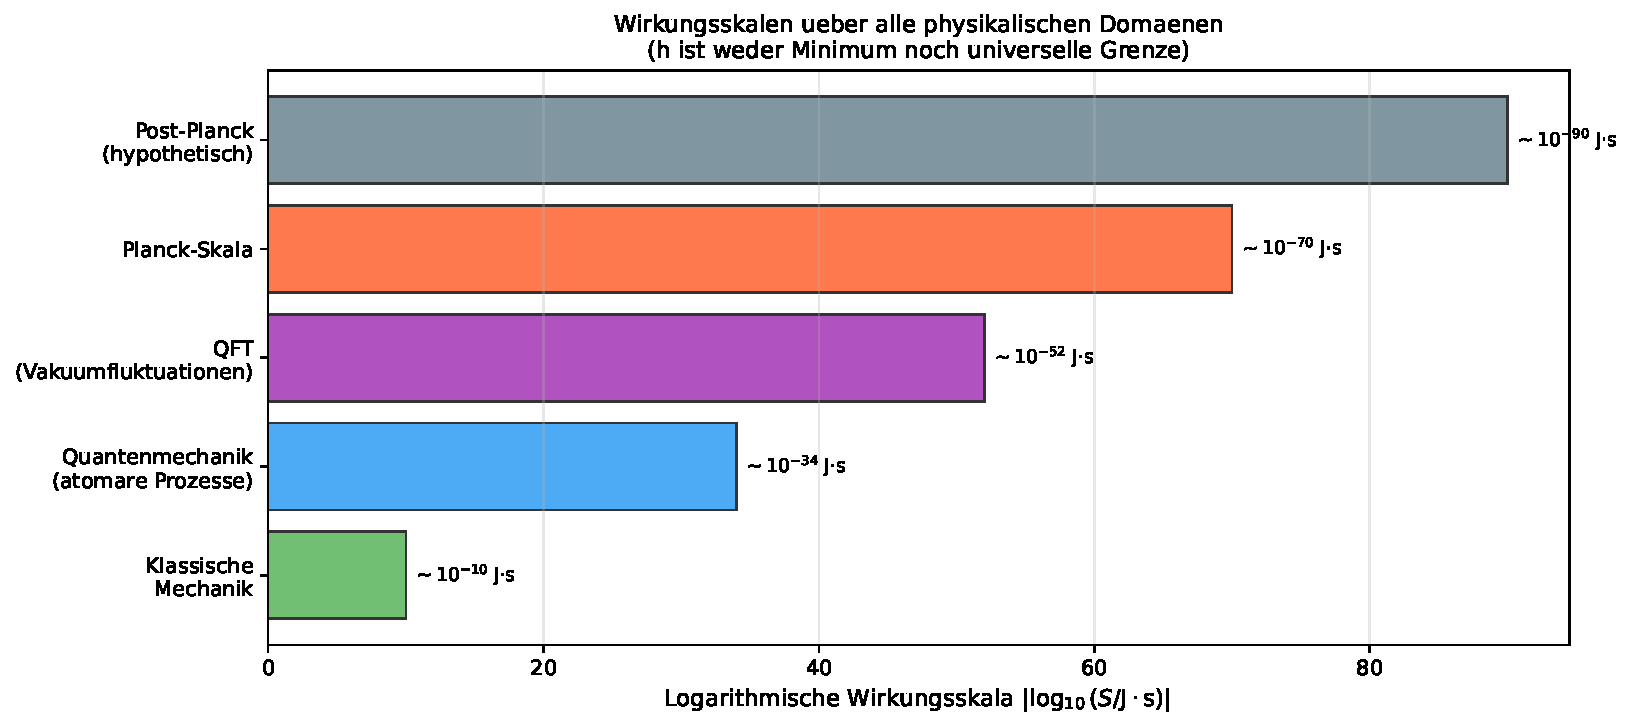
\includegraphics[width=0.9\textwidth]{fig5_skalen.pdf}
  \caption{Wirkungsskalen über alle physikalischen Domänen. $h$ markiert eine
    charakteristische Skala der atomaren Quantenmechanik, aber weder ein Minimum
    noch eine universelle Grenze physikalischer Wirkungen.}
  \label{fig:skalen}
\end{figure}

% ═════════════════════════════════════════════════════════════════════════════
\section{Zusammenfassung der Gegenbeispiele}
% ═════════════════════════════════════════════════════════════════════════════

\begin{table}[htbp]
  \centering
  \caption{Übersicht der Gegenbeispiele gegen die Fehldeutung von $h$ als Wirkungsminimum.}
  \label{tab:gegenbeispiele}
  \renewcommand{\arraystretch}{1.4}
  \begin{tabular}{>{\bfseries}p{3.2cm}p{5.5cm}p{4.5cm}}
    \toprule
    Kontext & Physikalischer Prozess & Wirkungsskala \\
    \midrule
    Klassische Mechanik &
      Makroskopisches Pendel mit Amplitude $\vartheta_0 \to 0$ &
      $S \to 0$, beliebig klein \\
    Feynman-Pfadintegral &
      Alle Pfade tragen zur Amplitude bei &
      $S[\gamma] \in \mathbb{R}$, kein Minimum \\
    Harmonischer Oszillator &
      Einzel-Photon-Emission bei $\omega_0 \to 0$ &
      $S_{\mathrm{Emission}} \ll h$ möglich \\
    Unschärferelation &
      Genauer Grenzwert ist $\hbar/2 = h/(4\pi)$ &
      $\sim h/12{,}6 \ll h$ \\
    QFT-Vakuum &
      Nullpunktsfluktuationen pro Mode &
      $S_0 \sim \hbar/2 < h$ \\
    Natürliche Einheiten &
      $h$ verschwindet; Wirkung ist dimensionslos &
      Kein privilegierter Wert \\
    \bottomrule
  \end{tabular}
\end{table}

% ═════════════════════════════════════════════════════════════════════════════
\section{Ausblick: Offene Fragen und tiefere Implikationen}
% ═════════════════════════════════════════════════════════════════════════════

\subsection{Die Planck-Skala als mögliche fundamentale Grenze}

Während $h$ selbst kein Wirkungsminimum darstellt, gibt es in der theoretischen Physik
ernsthafte Überlegungen, ob es eine \emph{fundamentale Längen- oder Wirkungsskala} gibt,
jenseits derer die beschreibenden Konzepte der Quantenmechanik und der allgemeinen
Relativitätstheorie zusammenbrechen. Die Planck-Länge ist definiert als
\begin{equation}
  \ell_P = \sqrt{\frac{\hbar G}{c^3}} \approx 1{,}616\times 10^{-35}\,\text{m},
\end{equation}
und die entsprechende Planck-Wirkung
\begin{equation}
  S_P = \hbar = \frac{h}{2\pi} \approx 1{,}055\times 10^{-34}\,\mathrm{J{\cdot}s}.
\end{equation}
Bemerkenswert: Die natürliche fundamentale Wirkungseinheit ist $\hbar$, nicht $h$. Und
auch $\hbar$ ist kein \emph{Minimum} im Sinne einer unüberwindlichen Schranke, sondern die
Einheit, in der Planck-skalige Prozesse natürlicherweise gemessen werden.

Die Stringtheorie~\cite{polchinski1998} und die Schleifenquantengravitation~\cite{rovelli2004}
legen nahe, dass unterhalb der Planck-Skala keine konsistente physikalische Beschreibung
existiert. Wenn überhaupt eine fundamentale Wirkungsschranke existiert, dann wäre sie
$S \gtrsim \hbar$ -- aber selbst diese Aussage ist in den meisten Quantengravitations-Ansätzen
nicht rigoros etabliert, sondern ein heuristisches Argument basierend auf der
Selbst-Energie-Divergenz der Gravitation.

\subsection{Minimale Länge und die Generalisierte Unschärferelation}

In der Quantengravitation wird häufig die sogenannte \emph{Generalisierte Unschärferelation}
(GUP, Generalized Uncertainty Principle) diskutiert~\cite{adler1999,maggiore1993}:
\begin{equation}
  \Delta x \cdot \Delta p \geq \frac{\hbar}{2}\left[1 + \beta\left(\frac{\Delta p}{m_P c}\right)^2\right],
  \label{eq:gup}
\end{equation}
wobei $\beta$ ein dimensionsloser Parameter der Größenordnung~1 ist und $m_P$ die
Planck-Masse bezeichnet. Diese Relation impliziert eine minimale Länge
\begin{equation}
  \Delta x_{\min} = \hbar \sqrt{\beta} / (m_P c) = \sqrt{\beta}\,\ell_P.
\end{equation}
Die GUP ist motiviert durch Gedankenexperimente in der Quantengravitation: Wenn man
ein Objekt auf die Planck-Skala lokalisieren möchte, muss man derart viel Energie
aufwenden, dass ein Schwarzes Loch entsteht -- was die Lokalisation verhindert. Falls
die GUP korrekt ist, folgt daraus eine effektive untere Schranke für
$\Delta x \cdot \Delta p$, die von der Planck-Skala gesetzt wird -- und nicht von $h$.

Es ist wichtig zu betonen, dass die GUP eine \emph{effektive} Beschränkung der
\emph{Messbarkeit} darstellt, keine Beschränkung der mathematischen Wirkung im
Pfadintegral. Selbst wenn es eine minimale messbare Länge gibt, folgt daraus nicht,
dass das Wirkungsintegral $S[\gamma]$ für alle Pfade durch $h$ nach unten beschränkt ist.

\subsection{Diskrete Raumzeit und das Problem der Wirkungsquantisierung}

Einige Ansätze zur Quantengravitation, insbesondere Causal Set Theory~\cite{bombelli1987}
und Spin-Foam-Modelle, postulieren eine fundamentale Diskretheit der Raumzeit auf der
Planck-Skala. In diesen Rahmen würde die klassische Wirkung $S[\gamma]$ aus
diskreten Beiträgen der Raumzeit-Atome zusammengesetzt:
\begin{equation}
  S_{\mathrm{diskret}} = \sum_{e \in \text{Kanten}} w(e),
\end{equation}
wobei $w(e)$ die Wirkung einer einzelnen Raumzeit-Kante ist. Falls die minimale
Kanten-Wirkung $w_{\min} = \hbar$ beträgt, wäre dies eine \emph{fundamentale Quantisierung
der Raumzeit-Wirkung} -- aber auch hier wäre das Quantum $\hbar$, nicht $h$.

Diese Frage bleibt offen und ist eines der tiefsten ungelösten Probleme der
theoretischen Physik. Die experimentellen Grenzen für Raumzeit-Diskretheit kommen aus
der Analyse von Gamma-Strahlen-Bursts~\cite{amelino2013}: Selbst hochenergetische Photonen
zeigen keine messbaren Dispersioneffekte, die auf eine Planck-skalige Raumzeit-Granularität
hinweisen würden -- zumindest auf dem aktuellen Messniveau.

\subsection{Die Rolle von $h$ in der Thermodynamik und Statistischen Mechanik}

Die Plancksche Konstante tritt in der Statistischen Mechanik in einer dritten, oft
übersehenen Rolle auf: als natürliche Phasenraumzellgröße~\cite{landau1980}. Im
klassischen Boltzmann-Formalismus hat die Zustandszahl im Phasenraum die Dimension
$[q \cdot p]^N$ und ist daher nicht dimensionslos. Planck normierte die Phasenraumzellgröße
auf $h^N$ (für $N$ Freiheitsgrade):
\begin{equation}
  Z = \frac{1}{N! h^{3N}} \int \mathrm{d}^{3N}q\,\mathrm{d}^{3N}p\,e^{-\beta H(q,p)}.
\end{equation}
Hier erscheint $h$ als \emph{normierendes Volumen einer Quantenzelle im Phasenraum}.
Diese Rolle ist konzeptuell verschieden von der Quantisierungsrolle in der
Wellenmechanik -- aber auch hier ist $h$ kein Minimum, sondern ein Maßstab.

Die statistische Bedeutung von $h$ wird besonders deutlich bei der Herleitung der
Sackur-Tetrode-Formel für die Entropie eines idealen Gases:
\begin{equation}
  S = Nk_B \left[\ln\!\left(\frac{V}{N}\left(\frac{4\pi m E}{3Nh^2}\right)^{3/2}\right) + \frac{5}{2}\right].
\end{equation}
Die Entropie divergiert klassisch logarithmisch mit $h \to 0$. Das ist das Gibbs'sche
Paradoxon in seiner tiefsten Form: Erst $h$ macht die Zustandsdichte endlich und die
Entropie extensive. Auch hier fungiert $h$ also als \emph{Regularisierungsskala}, nicht als Minimum.

\subsection{Post-Standardmodell-Physik: Könnte $h$ variabel sein?}

Eine faszinierende, wenn auch hochspekulative Frage betrifft die \emph{zeitliche
Konstanz} von $h$. Die Feinstrukturkonstante
\begin{equation}
  \alpha = \frac{e^2}{4\pi\varepsilon_0 \hbar c} \approx \frac{1}{137{,}036}
\end{equation}
hängt von $\hbar$, $c$ und $e$ ab. Messungen der Absorptionsspektren weit entfernter
Quasare bei verschiedenen Rotverschiebungen~\cite{webb2001,king2012} haben ergeben, dass
$\alpha$ möglicherweise über kosmologische Zeitskalen variiert (wobei die Evidenz umstritten ist).
Falls $\alpha$ variiert, dann muss mindestens eine der Konstanten $\hbar$, $c$ oder $e$ zeitlich
veränderlich sein. Szenarien mit variablem $\hbar$ wurden explizit untersucht
(z.\,B. im Rahmen von Brans-Dicke-artigen Theorien) und würden fundamentale Konsequenzen
für die Bedeutung des Wirkungsquantums haben:

\begin{itemize}[leftmargin=2em]
  \item Ein zeitlich variierendes $h$ würde bedeuten, dass die Quantisierungsskala
        kosmologisch nicht invariant ist.
  \item Das heutige Minimum der Heisenberg-Unschärfe ($\hbar/2$) wäre ein
        kosmologisch zeitabhängiger Wert.
  \item Die Planck-Skala selbst -- und damit jede Vorstellung einer fundamentalen
        Wirkungsgrenze -- würde zeitlich driften.
\end{itemize}

Aktuelle Experimente~\cite{uzan2011} setzen obere Grenzen von
$|\dot{h}/h| \lesssim 10^{-15}\,\text{yr}^{-1}$, was auf eine sehr große
Stabilität hindeutet -- aber theoretisch schließt keine bekannte Theorie eine
langsame Variation aus.

\subsection{Informationstheoretische Perspektive: $h$ als Informationsmaß}

Wheelers Programm ``It from Bit''~\cite{wheeler1990} und neuere Formulierungen des
Holographischen Prinzips~\cite{bousso2002} eröffnen eine informationstheoretische
Sichtweise auf $h$. In der holographischen Entropie-Schranke (Bekenstein-Bound) gilt
für ein System mit Energie $E$ und räumlicher Ausdehnung $R$:
\begin{equation}
  S_{\mathrm{ent}} \leq \frac{2\pi k_B E R}{\hbar c}.
\end{equation}
Hier tritt $\hbar$ als Konversionsfaktor zwischen Energie-Raum-Produkten und
Entropie (Information) auf. Die maximale Information, die in einer Raumzeit-Region
gespeichert werden kann, ist durch $\hbar$ reguliert.

Aus informationstheoretischer Sicht könnte $h$ als die \emph{minimale Wirkung pro Bit}
interpretiert werden, die benötigt wird, um Information physikalisch zu kodieren:
\begin{equation}
  h_{\mathrm{bit}} = \hbar \ln 2 \approx 0{,}693\,\hbar \approx 7{,}3\times 10^{-35}\,\mathrm{J{\cdot}s}.
\end{equation}
Dies ist die Landauer-Schranke für irreversible Informationsverarbeitung bei Temperatur
$T \to 0$, ausgedrückt als Wirkung. Auch hier: $h_{\mathrm{bit}} < h$. Selbst die
informationstheoretische Wirkungsschranke liegt \emph{unter} $h$.

\subsection{Konsequenzen für das Konzept der Quantengranularität}

Die in dieser Arbeit dargelegten Gegenbeispiele werfen eine tiefere Frage auf: Was
meinen wir eigentlich, wenn wir sagen, die Natur sei ``körnig''? Die Quantenmechanik
ist in zwei Sinnen diskret:

\begin{enumerate}[leftmargin=2em]
  \item \textbf{Energiequantisierung in gebundenen Systemen:} Gebundene Zustände haben
    diskrete Energiespektren. Das diskrete Spektrum ist eine Folge der Randbedingungen,
    nicht einer fundamentalen Unteilbarkeit der Energie.
  \item \textbf{Unschärfe komplementärer Observablen:} Die Heisenbergsche Unschärferelation
    verbietet gleichzeitige scharfe Messung von $x$ und $p$. Das ist eine
    \emph{epistemische} (oder ontologische, je nach Interpretation) Schranke.
\end{enumerate}

Beide Diskretheitseigenschaften sind in $h$ kodiert, aber keine bedeutet, dass die
Wirkung als Funktional diskret oder nach unten beschränkt ist. Die ``Körnigkeit'' der
Natur ist eine Eigenschaft von Messungen und Spektren, nicht von Trajektorien.

\subsection{Zusammenfassung des Ausblicks}

\begin{quote}
\textbf{Überblick der offenen Fragen:}
\begin{enumerate}[leftmargin=1.5em,label=\arabic*.]
  \item \textbf{Quantengravitation:} Gibt es eine fundamentale Wirkungsgrenze bei der
    Planck-Skala, oder ist auch dort das Wirkungsintegral kontinuierlich?
  \item \textbf{Minimale Länge (GUP):} Falls es eine minimale messbare Länge gibt,
    welche Konsequenz hat das für die Wirkungsskala physikalischer Prozesse?
  \item \textbf{Diskrete Raumzeit:} Falls Spin-Foam- oder Causal-Set-Modelle korrekt
    sind: Was ist die kleinste Wirkungseinheit eines Raumzeit-Atoms?
  \item \textbf{Variabilität von $\hbar$:} Ist $h$ kosmologisch konstant? Welche
    Messkonzepte könnten eine Variation nachweisen?
  \item \textbf{Informationstheorie:} Ist die Landauer-Schranke $\hbar\ln 2$ die
    eigentliche tiefste physikalische Wirkungsgrenze?
  \item \textbf{Interpretation:} In welchem Sinne ist die Natur ``körnig'' -- und in
    welchem Sinne nicht?
\end{enumerate}
\end{quote}

% ═════════════════════════════════════════════════════════════════════════════
\section{Schluss}
% ═════════════════════════════════════════════════════════════════════════════

Das Plancksche Wirkungsquantum $h$ ist eine der fundamentalsten Konstanten der Physik
und markiert den Übergang von der klassischen zur Quantenwelt. Aber es ist kein
Minimum der physikalischen Wirkung -- weder im klassischen noch im quantenmechanischen
Formalismus. Wirkungsintegrale können jeden reellen Wert annehmen; Vakuumfluktuationen
besitzen Wirkungen kleiner als $h$; die Heisenbergsche Unschärferelation hat die Schranke
$\hbar/2$, nicht $h$; und das Feynman-Pfadintegral integriert über Pfade beliebiger
Wirkung.

Die korrekte physikalische Bedeutung von $h$ ist die eines \emph{Quantisierungsmaßes}:
Es definiert das Intervall, in dem periodische Aktionsvariablen diskrete Werte annehmen,
und gibt die natürliche Phasenraumzellgröße der statistischen Mechanik an. Diese
präzisere Formulierung ist nicht nur akademisch korrekt -- sie öffnet den Blick für
tiefere Fragen über die Natur von Diskretheit, Minimalskalen und die Rolle von $h$ in
der noch ausstehenden Theorie der Quantengravitation.

Die Fehldeutung von $h$ als absolutem Wirkungsminimum ist pädagogisch verständlich,
aber sie verstellt den Blick auf die eigentliche physikalische Tiefe der Konstante.
$h$ ist das Maß der Quantenwelt -- nicht ihre Grenzwand.

% ─────────────────────────────────────────────────────────────────────────────
\bibliographystyle{plain}
\begin{thebibliography}{99}

\bibitem{planck1900}
M. Planck, ``Über eine Verbesserung der Wienschen Spektralgleichung,''
\textit{Verhandlungen der Deutschen Physikalischen Gesellschaft}, \textbf{2}, 202--204 (1900).

\bibitem{bohr1913}
N. Bohr, ``On the Constitution of Atoms and Molecules,''
\textit{Philosophical Magazine}, \textbf{26}(151), 1--25 (1913).

\bibitem{sommerfeld1916}
A. Sommerfeld, ``Zur Quantentheorie der Spektrallinien,''
\textit{Annalen der Physik}, \textbf{356}(17), 1--94 (1916).

\bibitem{feynman1948}
R.~P. Feynman, ``Space-Time Approach to Non-Relativistic Quantum Mechanics,''
\textit{Reviews of Modern Physics}, \textbf{20}(2), 367--387 (1948).

\bibitem{heisenberg1927}
W. Heisenberg, ``Über den anschaulichen Inhalt der quantentheoretischen Kinematik und
Mechanik,'' \textit{Zeitschrift für Physik}, \textbf{43}, 172--198 (1927).

\bibitem{polchinski1998}
J. Polchinski, \textit{String Theory}, 2 vols. Cambridge University Press (1998).

\bibitem{rovelli2004}
C. Rovelli, \textit{Quantum Gravity}. Cambridge University Press (2004).

\bibitem{adler1999}
R.~J. Adler, D.~I. Santiago, ``On gravity and the uncertainty principle,''
\textit{Modern Physics Letters A}, \textbf{14}(20), 1371--1381 (1999).

\bibitem{maggiore1993}
M. Maggiore, ``A generalized uncertainty principle in quantum gravity,''
\textit{Physics Letters B}, \textbf{304}(1--2), 65--69 (1993).

\bibitem{bombelli1987}
L. Bombelli, J. Lee, D. Meyer, R. Sorkin, ``Space-time as a causal set,''
\textit{Physical Review Letters}, \textbf{59}(5), 521--524 (1987).

\bibitem{amelino2013}
G. Amelino-Camelia, ``Quantum-spacetime phenomenology,''
\textit{Living Reviews in Relativity}, \textbf{16}, 5 (2013).

\bibitem{landau1980}
L.~D. Landau, E.~M. Lifshitz, \textit{Statistical Physics}, 3rd ed.
Pergamon Press, Oxford (1980).

\bibitem{webb2001}
J.~K. Webb \textit{et al.}, ``Further evidence for cosmological evolution of the fine
structure constant,'' \textit{Physical Review Letters}, \textbf{87}(9), 091301 (2001).

\bibitem{king2012}
J.~A. King \textit{et al.}, ``Spatial variation in the fine-structure constant,''
\textit{Monthly Notices of the Royal Astronomical Society}, \textbf{422}(4), 3370--3414 (2012).

\bibitem{uzan2011}
J.-P. Uzan, ``Varying constants, gravitation and cosmology,''
\textit{Living Reviews in Relativity}, \textbf{14}, 2 (2011).

\bibitem{wheeler1990}
J.~A. Wheeler, ``Information, physics, quantum: The search for links,'' in
\textit{Complexity, Entropy, and the Physics of Information}, W.~H. Zurek (ed.),
Addison-Wesley, 3--28 (1990).

\bibitem{bousso2002}
R. Bousso, ``The holographic principle,''
\textit{Reviews of Modern Physics}, \textbf{74}(3), 825--874 (2002).

\end{thebibliography}

\end{document}
